\documentclass[conference]{IEEEtran}

\usepackage{cite}
\usepackage{amsmath,amssymb}
\usepackage{graphicx}
\usepackage{booktabs}
\usepackage{url}

\begin{document}

\title{TCN-BiGRU and XGBoost-Based Near-Failure Detection for Aircraft Turbofan Engines}

\author{
\IEEEauthorblockN{Author One, Author Two, Author Three}
\IEEEauthorblockA{
Department / Faculty / University\\
City, Country\\
email@example.com}
}

\maketitle

\begin{abstract}
Predictive maintenance of aircraft engines requires accurate identification of near-failure operating states from multivariate sensor sequences. This study proposes a hybrid TCN-BiGRU + XGBoost approach for near-failure detection using the NASA C-MAPSS turbofan engine degradation dataset. The proposed model first extracts local temporal degradation patterns using causal temporal convolutional network (TCN) blocks, then models bidirectional long-range temporal dependencies using a BiGRU layer and attention pooling. The learned embedding is finally classified by XGBoost to distinguish normal and near-failure engine states. Experiments are conducted on all four C-MAPSS subsets, FD001--FD004. The proposed method achieves an average F1-score of 0.9089, average ROC-AUC of 0.9941, and average PR-AUC of 0.9815 across the four datasets.
\end{abstract}

\begin{IEEEkeywords}
predictive maintenance, turbofan engine, C-MAPSS, TCN, BiGRU, XGBoost, anomaly detection, remaining useful life
\end{IEEEkeywords}

\section{Introduction}

Aircraft engine reliability is a critical requirement for operational safety, maintenance planning, and cost reduction. Modern turbofan engines are monitored using multivariate sensor streams that reflect changes in pressure, temperature, speed, and other operating conditions. As degradation progresses, these sensor signals contain temporal patterns that can be used to identify near-failure behavior before complete engine failure occurs.

Traditional maintenance strategies rely on scheduled inspections or rule-based thresholds. However, fixed thresholds may not capture complex nonlinear degradation patterns, especially when operating conditions and fault modes vary across engines. Data-driven predictive maintenance methods address this limitation by learning degradation signatures directly from historical sensor data.

The NASA C-MAPSS dataset is widely used for evaluating prognostics and health management algorithms. It contains run-to-failure simulations for turbofan engines under different operating conditions and fault modes. Most studies formulate the task as remaining useful life (RUL) regression, but near-failure detection is also important because maintenance decisions are often made as binary or multi-class health-state decisions.

This paper proposes a hybrid TCN-BiGRU + XGBoost architecture for near-failure detection. In the proposed approach, TCN layers capture local temporal degradation patterns, BiGRU layers model forward and backward temporal dependencies, attention pooling produces a compact engine health embedding, and XGBoost performs the final classification. The binary target is defined as near failure when RUL $< 30$ cycles and normal otherwise.

The main contributions of this study are:
\begin{itemize}
    \item FILL: Contribution 1.
    \item FILL: Contribution 2.
    \item FILL: Contribution 3.
\end{itemize}

\section{Related Work}

Deep learning has been widely applied to turbofan engine prognostics using the C-MAPSS dataset. Recurrent neural networks such as LSTM and GRU models are commonly used because engine degradation is sequential in nature. Attention-based recurrent models further improve interpretability and temporal weighting by allowing the model to focus on informative time steps.

Temporal convolutional networks have also been used for time-series modeling because dilated causal convolutions can capture local and medium-range temporal dependencies efficiently. Transformer-based methods and PatchTST-style architectures have recently been applied to time-series classification and RUL prediction. Gradient boosting methods such as XGBoost remain strong classifiers for structured representations.

FILL: Add literature citations and compare the proposed method with prior methods.

\section{Dataset and Problem Definition}

\subsection{C-MAPSS Dataset}

The experiments use the NASA C-MAPSS turbofan engine degradation dataset. It contains four subsets: FD001, FD002, FD003, and FD004. These subsets differ in the number of operating conditions and fault modes.

\begin{table}[!t]
\centering
\caption{NASA CMAPSS dataset characteristics.}
\label{tab:dataset\_characteristics}
\begin{tabular}{lccccccc}
\hline
Dataset & Train engines & Test engines & Train samples & Test samples & Conditions & Fault modes & Fault type \\
\hline
FD001 & 100 & 100 & 20631 & 13096 & 1 & 1 & HPC degradation \\
FD002 & 260 & 259 & 53759 & 33991 & 6 & 1 & HPC degradation \\
FD003 & 100 & 100 & 24720 & 16596 & 1 & 2 & HPC and fan degradation \\
FD004 & 249 & 248 & 61249 & 41214 & 6 & 2 & HPC and fan degradation \\
\hline
\end{tabular}
\end{table}


\subsection{Label Definition}

For each training engine, RUL is computed as
\begin{equation}
RUL_i(t) = T_i - t,
\end{equation}
where $T_i$ is the final cycle of engine $i$ and $t$ is the current cycle. The binary label is defined as
\begin{equation}
y =
\begin{cases}
1, & RUL < 30 \\
0, & RUL \geq 30.
\end{cases}
\end{equation}

FILL: Explain why the 30-cycle threshold is selected.

\section{Proposed Method}

\begin{figure}[!t]
\centering
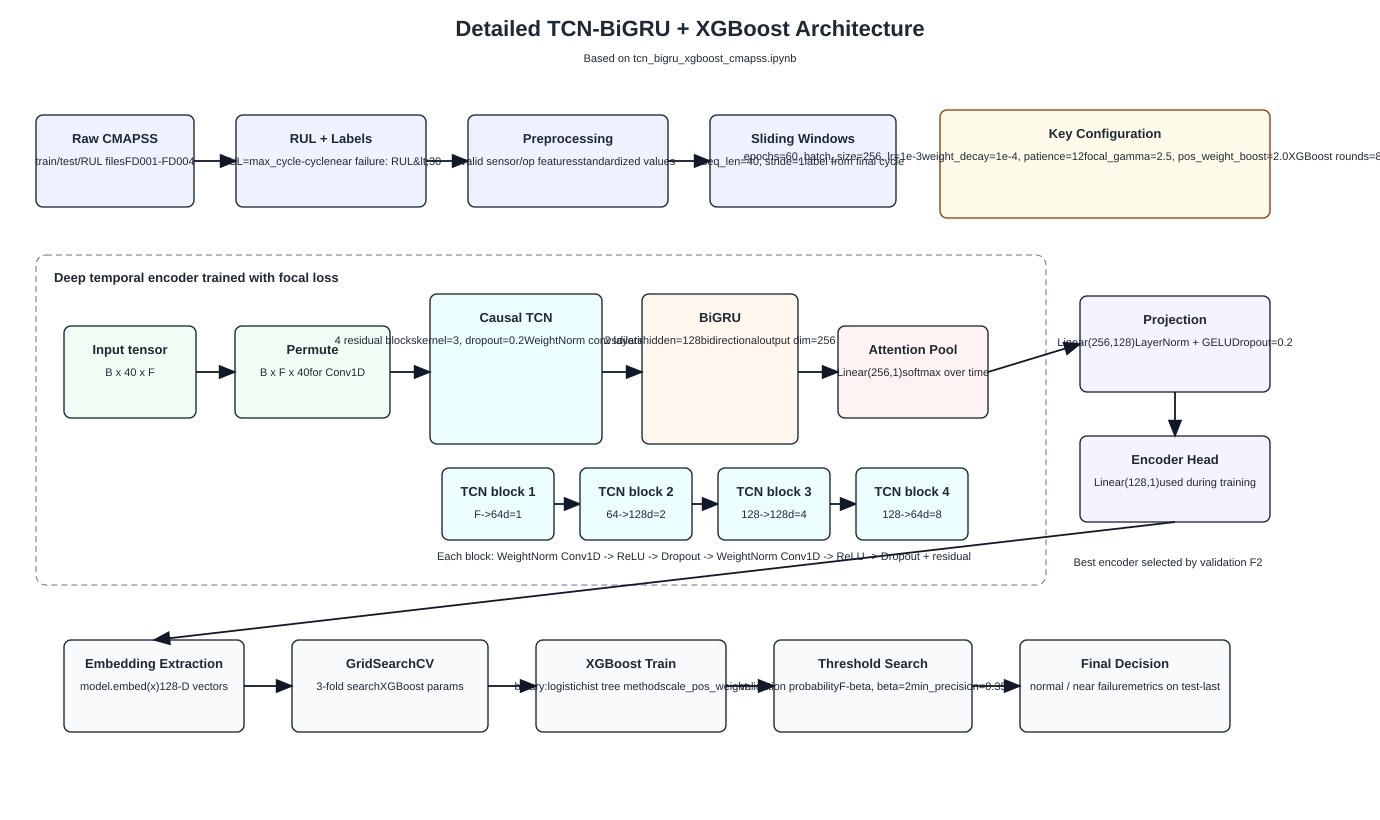
\includegraphics[width=\linewidth]{figures/fig_tcn_bigru_xgboost_architecture_detailed.svg}
\caption{Overall architecture of the TCN-BiGRU + XGBoost near-failure detection pipeline.}
\label{fig:architecture}
\end{figure}

\subsection{Sliding Window Generation}

Each engine trajectory is converted into fixed-length temporal windows. A window contains sensor and operating-condition measurements over consecutive cycles. The model uses a sequence length of 40 cycles. Each window is assigned the label of its final time step.

FILL: Add exact preprocessing details: selected sensors, normalization method, stride, and train-validation split.

\subsection{TCN Feature Extraction}

The first stage uses causal TCN blocks with dilated convolutions. These layers learn local degradation patterns while preserving temporal order. The TCN channel configuration is [64, 128, 128, 64], with residual connections and weight normalization.

\subsection{BiGRU Temporal Modeling}

The TCN output is passed to a bidirectional GRU. The BiGRU models temporal dependencies in both forward and backward directions over the extracted TCN features.

\subsection{Attention Pooling and XGBoost Classification}

Attention pooling converts the sequence of BiGRU hidden states into a fixed-length 128-dimensional embedding. The learned embedding is used as input to an XGBoost binary classifier. A validation-optimized probability threshold converts classifier probabilities into normal or near-failure predictions.

\begin{table}[!t]
\centering
\caption{Main hyperparameters of TCN-BiGRU + XGBoost.}
\label{tab:hyperparameters}
\begin{tabular}{lc}
\hline
Hyperparameter & Value \\
\hline
Sequence length & 40 cycles \\
Batch size & 256 \\
Epochs & 60 \\
Patience & 12 \\
Learning rate & 1e-3 \\
Weight decay & 1e-4 \\
Focal gamma & 2.0 \\
TCN channels & [64, 128, 128, 64] \\
GRU hidden size & 128 bidirectional \\
GRU layers & 2 \\
GRU dropout & 0.30 \\
Embedding size & 128 \\
XGBoost rounds & 800 \\
XGBoost learning rate & 0.03 \\
XGBoost max depth & 6 \\
XGBoost subsample & 0.8 \\
XGBoost colsample\_bytree & 0.8 \\
XGBoost min\_child\_weight & 5 \\
XGBoost early stopping & 40 rounds \\
\hline
\end{tabular}
\end{table}


\section{Experimental Setup}

All experiments are conducted on FD001--FD004. The evaluation uses the final available test sequence for each engine, corresponding to a realistic decision point where the latest engine state is classified as normal or near failure.

The reported metrics are precision, recall, F1-score, ROC-AUC, PR-AUC, and specificity. The F1-score is emphasized because the near-failure class is imbalanced and both missed failures and false alarms are important.

FILL: Add hardware/software details, random seed, library versions, and training time if available.

\section{Results and Discussion}

\subsection{Proposed Method Results}

The proposed TCN-BiGRU + XGBoost model achieves strong results across all CMAPSS subsets. The mean F1-score is 0.9089, the mean ROC-AUC is 0.9941, and the mean PR-AUC is 0.9815.

\input{tables/proposed_tcn_bigru_xgboost_results.tex}

\begin{figure}[!t]
\centering
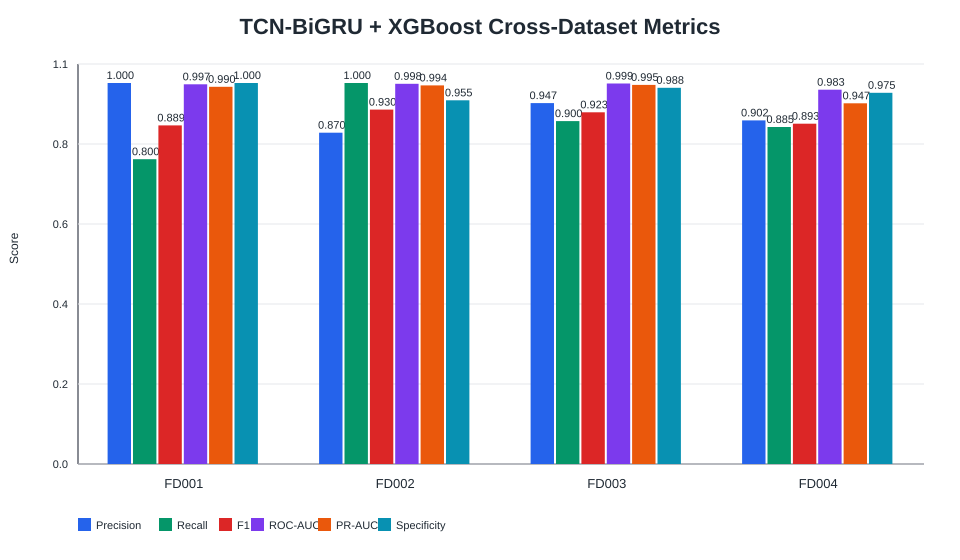
\includegraphics[width=\linewidth]{figures/fig_proposed_cross_dataset_metrics.svg}
\caption{Cross-dataset precision, recall, F1-score, ROC-AUC, PR-AUC, and specificity of the proposed method.}
\label{fig:proposed_metrics}
\end{figure}

The highest F1-score is obtained on FD002, while FD004 remains challenging because it combines multiple operating conditions with two fault modes. The high ROC-AUC values across all subsets show that the model ranks near-failure samples well even when the classification threshold changes.

\subsection{Confusion Matrix Analysis}

\begin{figure}[!t]
\centering
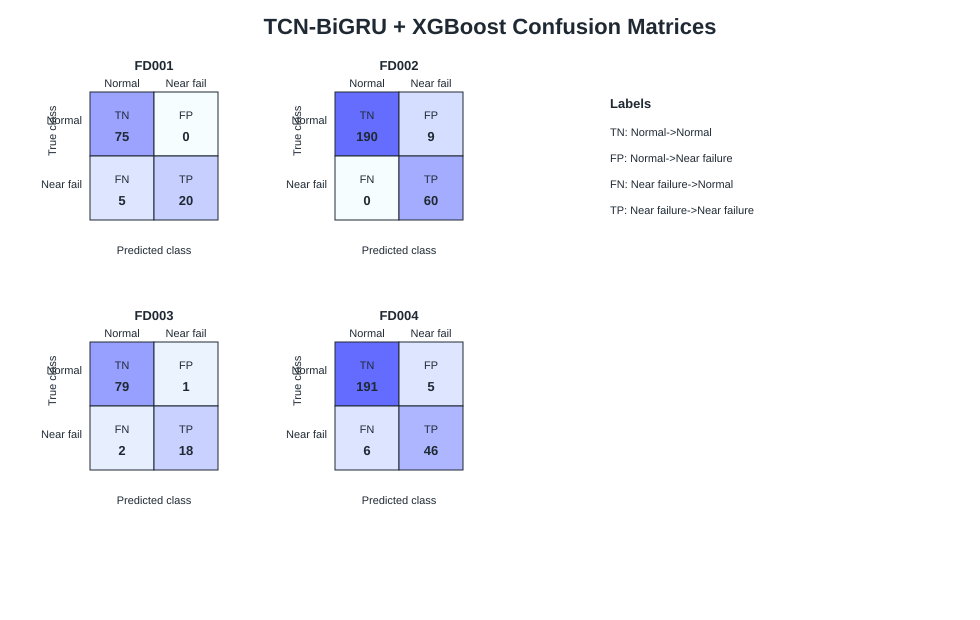
\includegraphics[width=\linewidth]{figures/fig_proposed_confusion_matrices.svg}
\caption{Confusion matrices of the proposed method on the final test sequence of each engine.}
\label{fig:confusion}
\end{figure}

The confusion matrices show the trade-off between false alarms and missed near-failure engines. FD001 achieves perfect precision, while FD002 achieves perfect recall.

\subsection{Comparison with Other Methods}

\input{tables/method_comparison_f1.tex}

\begin{figure}[!t]
\centering
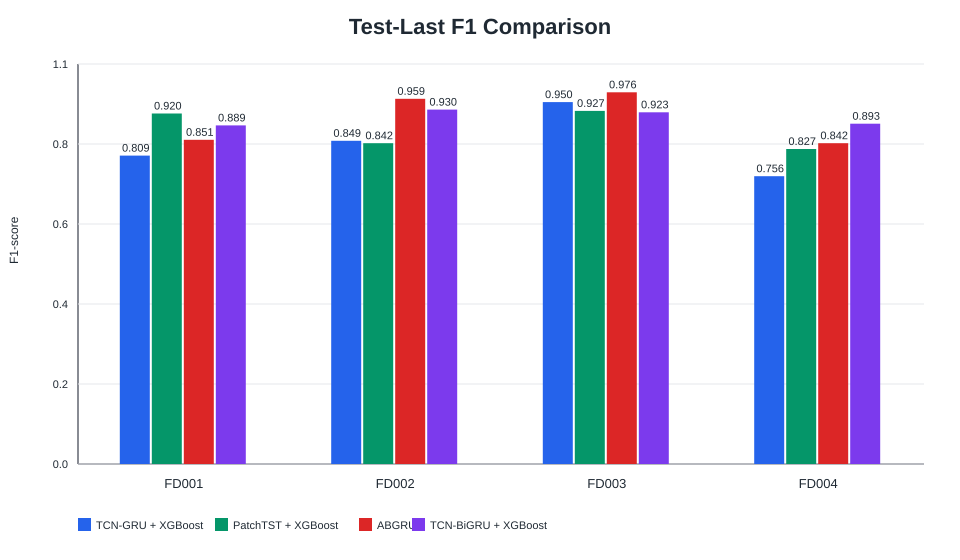
\includegraphics[width=\linewidth]{figures/fig_method_comparison_f1.svg}
\caption{Test-last F1-score comparison across CMAPSS subsets.}
\label{fig:f1_comparison}
\end{figure}

The proposed method obtains the best average F1-score among the compared methods. However, ABGRU performs slightly better on FD002 and FD003. Therefore, the main claim should be written as average cross-dataset improvement, not superiority on every individual dataset.

\subsection{Architecture Discussion}

\begin{table}[!t]
\centering
\caption{Architectural differences between the prior TCN-GRU baseline and TCN-BiGRU method.}
\label{tab:architecture\_comparison}
\begin{tabular}{lcc}
\hline
Component & TCN-GRU + XGBoost & TCN-BiGRU + XGBoost \\
\hline
Topology & Parallel TCN and GRU branches & Sequential TCN $\rightarrow$ BiGRU $\rightarrow$ attention \\
TCN normalization & BatchNorm1d & WeightNorm \\
TCN channels & [64, 128, 128] & [64, 128, 128, 64] \\
Recurrent unit & Bidirectional GRU, hidden 64 & Bidirectional GRU, hidden 128 \\
Window length & 30 cycles & 40 cycles \\
Deep embedding & 128 dimensions & 128 dimensions \\
XGBoost input & Embedding + handcrafted statistics & Embedding only \\
Early stopping & Validation loss & Validation F1 \\
\hline
\end{tabular}
\end{table}


Compared with the prior TCN-GRU + XGBoost baseline, the proposed model uses a sequential architecture in which the TCN first extracts local temporal features and the BiGRU then models temporal dependencies over those features. This design provides a hierarchical representation of degradation behavior.

\section{Conclusion}

This study presented a hybrid TCN-BiGRU + XGBoost method for near-failure detection in aircraft turbofan engines. The model combines causal temporal convolution, bidirectional recurrent modeling, attention pooling, and gradient-boosted classification. Experiments on all four C-MAPSS subsets demonstrate strong classification performance, with an average F1-score of 0.9089 and average ROC-AUC of 0.9941. The results suggest that sequential TCN-BiGRU feature learning provides a robust representation for engine health-state classification.

Future work will investigate FILL: multi-class health-state classification, RUL regression, explainability, real-time deployment, or uncertainty estimation.

\begin{thebibliography}{00}

\bibitem{cmapss}
A. Saxena, K. Goebel, D. Simon, and N. Eklund, ``Damage propagation modeling for aircraft engine run-to-failure simulation,'' in \emph{Proc. Int. Conf. Prognostics and Health Management}, 2008.

\bibitem{tcn}
FILL: TCN reference.

\bibitem{gru}
FILL: GRU/BiGRU reference.

\bibitem{xgboost}
FILL: XGBoost reference.

\bibitem{patchtst}
FILL: PatchTST or transformer time-series reference.

\bibitem{predictive-maintenance}
FILL: Recent aircraft predictive maintenance reference.

\end{thebibliography}

\end{document}
